% \documentclass[]{amsbook}
\documentclass[]{article}

% \input MyMacros.tex

\usepackage{graphicx}% Include figure files
\usepackage{dcolumn}% Align table columns on decimal point
\usepackage{bm}% bold math
% \usepackage{pictex}%
\usepackage{verbatim} % this is needed for \begin{comment} ... \end{comment}
\usepackage{lscape} % this is needed for occasional landscape figures
\usepackage{amsmath}
% \usepackage{appendix}
% \usepackage{subfigure}
\usepackage{epsfig}
\usepackage{amsfonts}
\usepackage[margin=1.1in, top=1.1in, bottom=1.1in]{geometry}

% \textwidth 550pt
% \textheight 500pt
% \hoffset -3.5cm
\def\betabold{{\pmb{$\beta$}}}

\setcounter{tocdepth}{3}
%
\begin{document}

\date{August 26, 2923}

% \voffset=1.5
\title{
\centerline{}
\centerline{}
\centerline{}
ETEAPOT PTR Benchmark-II: \\
Transfer Matrices and Twiss Functions 
}
\author{J. D. Talman and R. M. Talman
}

\maketitle

% \tableofcontents

\begin{abstract}
In this chapter
ETEAPOT is used to obtain transfer matrices between arbitrary lattice positions,
and, from them, Twiss functions as functions of longitudinal coordinate $s$.
Three new PTR sxf files now replace three benchmark lattices processed in
the  November 6, 2019, ``ETEAPOT EDM Benchmark I: Updated Results for Proton 
EDM Benchmark Lattices''.  The lattices have field indices 
$m=0.29447$,  $m=0.32349$, and $m=0.39447$, which represent a much reduced
range of electrode shapes than the earlier report (as well as corresponding to the
PTR ``predominantly electric lattice'' rather than the ``proton EDM lattice'').
Once-around transfer matrices are obtained and used to determine beta functions 
at the origin as well as transverse tunes.  In Benchmark~I, tunes have been obtained 
using multiturn tracking (thereby avoiding aliasing ambiguity) but general transfer matrices 
and beta functions were not obtained and the issue of aliasing ambiguities affecting the 
determination of integer tune values was only mentioned.  This report addresses these
deficiencies.  Results are compared to values obtained from a linearized MAPLE 
transfer matrix BSM formalism. In all cases the lumped quadrupole strengths have been
reduced to a common (small enough to be relatively unimportant) value for which the 
vertical betatron motion is conservatively stable.  
\end{abstract}
%

\section{Determination of Twiss Functions From Transfer Matrices}
Table ~\ref{tbl:benchmarkParams.1} contains PTR position and length parameters as well as tune values 
obtained in the PTR-Benchmark-I report.   The ``same'' three lattices that were processed in the PTR
Benchmark-I  report are processed in this  PTR-Benchmark-II report.  The reason for ``same'' to be
in quotation marks is that, though the geometrry is identical, and very weak, the quadrupole strengths
are not identical in Benchmark-I and Benchmark-II.  This complication is brought about by the
newly introduced concept of ``compromise quadrupoles'' which need to be employed for 
``predominantly electric bending'' for which some quads are electric, some magnetic.

 An important peripheral role for this PTR-Benchmark-II report is to bring the UAL:PTR and MAPLE:PTR
results into conformity.  Historically the UAL:ETEAPOT code, folowing formulas of Mu\~noz and 
Pavic\cite{Munoz}, was based on relativistically valid analytical solutions of orbits in the 
Kepler/Coulomb/Spherical, inverse square law central force. The toroidal shape parameter for this
potential is $m=1.0$.  Some ETEAPOT tracking formulas, mainly concerned with longitudinal 
(i.e. time-dependent) orbiitry, for general values of $m\_nom$, rely on perturbative expansions relative
to $m\_nom=1.0$.  

According to PTR analyses using MAPLE:BSM, the ``sweet-spot'' for predominantly electric storage rings
is $m=0.32349$.  The presence of superimposed magnetic bending in ETEAPOT, can therefore
also be perturbative, with ``small deviation'' being $\eta_M/\eta_E$, typically within the range +/-0.1.  





\clearpage



\section{Analysis of the Once-Around Transfer Matrix at the Origin}
In this section $x$ and $y$ and $ct$ subscripts will be suppressed,
and only transverse evolution is to be discussed. 
The most general
transfer matrix is a six-by-six matrix ${\bf M}(s_i,s_j)$, which propagates a
phase space vector ${\bf x}(s_i)$ at $s_i$, to its value ${\bf x}(s_j)$ at $s_j$;
%
\begin{equation}
{\bf x}(s_j) 
 =
{\bf M}(s_i,s_j)\,
{\bf x}(s_i). 
\label{TM.1}
\end{equation}
%
ETEAPOT starts by assigning coordinates at the origin, $s_0=0$,
to the particles in a standard bunch (as described earlier), and then
evolves the standard bunch and records the coordinates ${\bf x}(s_i)$ 
at all points $s_i$.  From these results the transfer matrices 
${\bf M}(0,s_i)$ can be calculated (also as described earlier). By definition
%
\begin{equation}
{\bf M}(0,0)
 =
{\bf I}, 
\label{TM.2}
\end{equation}
%
where ${\bf I}$ is the $6\times6$ identity matrix. 

To extract Twiss lattice functions one needs periodic, ``once-around'' transfer 
matrices, distinguished by overhead tildes, and defined by
%
\begin{equation}
{\widetilde{\bf M}}(s_i)
 \equiv
{\bf M}(s_i,s_i+\mathcal{C}_0)
 =
{\bf M}(0,s_i)\,
{\bf M}(s_i,\mathcal{C}_0).
\label{TM.3}
\end{equation}
%
where $\mathcal{C}_0$ is the circumference of the design
orbit; the final step has been taken because knowledge of
$s_i+\mathcal{C}_0$ requires tracking for more than one
complete turn, but we are assuming that tracking has been
done only for exactly one complete turn. Propagation from
$s=\mathcal{C}_0$ to $\mathcal{C}_0+s_i$ is the same as
propagation from $s=0$ to $s_i$. The Twiss parameterization of 
(one partitioned diagonal
$2\times2$ block of) such a once-around, symplectic 
transfer matrix is
%
\begin{equation}
{\widetilde{\bf M}}(s_i)
 =
\begin{pmatrix}
\cos\mu + \alpha\sin\mu          & \beta\sin\mu \\
-\frac{1+\alpha^2}{\beta}\sin\mu & \cos\mu - \alpha\sin\mu 
\end{pmatrix}.
\label{TM.4}
\end{equation}
%
Extraction of the $\alpha_0$ and $\beta_0$, the Twiss parameters 
at the origin, can start from
%
\begin{equation}
\cos\mu
 = 
\frac{1}{2}\,\big({\widetilde{\bf M}}_{11}(0) + {\widetilde{\bf M}}_{22}(0)\big),
\label{TM.5}
\end{equation}
%
which fixes $\cos\mu$. Because of sign ambiguity, this determines only
$|\sin\mu|$. One also has the relations
%
\begin{equation}
\beta_0
 = 
\bigg|
\frac{\widetilde{\bf M}_{12}(0)}{\sin\mu}
\bigg|.
\label{TM.6}
\end{equation}
%
and
%
\begin{equation}
\alpha_0
 = 
\frac{1}{2\sin\mu}\,
\big({\widetilde{\bf M}}_{11}(0) - {\widetilde{\bf M}}_{22}(0)\big).
\label{TM.7}
\end{equation}
%
With $\beta$ being positive by convention, 
from the 1,2 element, sign($\sin\mu$) can be seen to be
the same as sign(${\widetilde{\bf M}}_{12}$). With $\cos\mu$ known,
this fixes $\sin\mu$.
Together, these relations fix $\sin\mu$, $\cos\mu$, $\alpha_0$, and $\beta_0$.

Conventionally one also introduces a third Twiss parameter
%
\begin{equation}
\gamma_0
 = 
\frac{1+\alpha_0^2}{\beta_0},
\label{TM.8}
\end{equation}
%
which can be obtained once $\beta_0$ and $\alpha_0$
have been determined. 

Because of the multiple-valued nature of inverse trig functions,
these relations do not determine a unique value for $\mu$. They do,
however, determine the quadrant in phase space in which the angle $\mu$
resides. For sign($\sin\mu$)$>$0 the angle $\mu$ resides in the first
or second quadrant, in which case the fractional tune is less than 1/2;
otherwise the fractional tune is greater than 1/2.
For sign($\cos\mu$)$>$0 the angle $\mu$ resides in the first
or fourth quadrant, in which case the fractional tune is below 1/4
or above 3/4. These considerations fix the fractional parts of
the tunes.

An ``aliasing'' or ``integer-tune'' ambiguity remains, however,
which cannot, even in principle, be obtained from the once-around 
matrix. Only if both transverse tunes are less than 1 (which is 
hardly ever the
case) would the tunes be equal to the fractional tunes that have
been determined. In general, to obtain the integer tunes, it is 
necessary to analyse the turn by turn data at sufficiently closely-space 
intermediate points in the lattice, or for multiple turns. (See examples in the previous chapter.)

\section{Evolving the Twiss Functions Around the Ring}
To find the Twiss parameters at an arbitrary location $s_i$ in the
ring requires the once-around transfer matrix ${\widetilde{\bf M}}(s_i)$. 
This can obtained most compactly by multiplying the equation
%
\begin{equation}
{\bf M}(0,s_j)
 =
{\bf M}(s_i,s_j)\,{\bf M}(0,s_i)
\label{TM.9}
\end{equation}
%
on the right by ${\bf M}^{-1}(0,s_i)$ to produce
%
\begin{equation}
{\bf M}(s_i,s_j)
 =
{\bf M}(0,s_j)\,{\bf M}^{-1}(0,s_i).
\label{TM.10}
\end{equation}
%
Substituting this with $s_j=\mathcal{C}_0$ into Eq.~(\ref{TM.3}) 
produces
%
\begin{equation}
\widetilde{\bf M}(s_i)
 =
{\bf M}(0,s_i)\,\widetilde{\bf M}(0)\,{\bf M}^{-1}(0,s_i).
\label{TM.11}
\end{equation}
%
Having obtained ${\widetilde{\bf M}}(s_i)$,
the procedure described in the previous subsection can
then be used to obtain $\alpha(s_i)$ and $\beta(s_i)$.
But the integer tune ambiguity can, again, not be
resolved. To resolve this ambiguity both $x$ and $y$ phases
have to be tracked continuously through the lattice,
requiring that they advance continuously and monotonically.
(Later, at least in principle, the same ambiguity will 
have to be faced for longitudinal motion. But the
integer longitudinal tune is almost always zero, so the
problem is usually absent in the longitudinal case.)

ETEAPOT requires the lattice description to be in the form
of an {\tt .sxf} file.  To be ``legal'' the granularity of such
a file has to be fine enough that no phase can advance by more
than a quarter integer through any element in the file. Before
working out the $\alpha$ and $\beta$ function evolution, 
ETEAPOT first works out the total phase advances from
the origin to every node specified by the {\tt .sxf} file
(or, if some elements are sliced more finely, by every node
after slicing). 

There is an alternative way of finding the betatron phase
advances. It starts with a Twiss parameterization
of ${\bf M}(0,s)$ from the origin to an arbitrary position $s$
in the lattice;
%
\begin{equation}
{\bf M}(0, s)
 =
\begin{pmatrix}
\sqrt{\frac{\beta(s)}{\beta_0}}\Big(\cos\psi(s) + \alpha_0\sin\psi(s)\Big) & 
            \sqrt{\beta_0\beta(s)}\,\sin\psi(s)                         \\
   \cdot & 
\sqrt{\frac{\beta_0}{\beta(s)}}\Big(\cos\psi(s) - \alpha(s)\sin\psi(s)\Big)         
\end{pmatrix}.
\label{TM.15}
\end{equation}
%
The 2,1 element is quite complicated; it is not shown here since it will not be needed
for the following analysis. Dividing the 1,1 element by the 1,2 element produces
%
\begin{equation}
\frac{{\bf M}_{1,1}(0, s)}{{\bf M}_{1,2}(0, s)}
 =
\frac{\sqrt{\frac{\beta(s)}{\beta_0}}\Big(\cos\psi(s) + \alpha_0\sin\psi(s)\Big)}
     {\sqrt{\beta_0\beta(s)}\,\sin\psi(s)}
 =
\frac{\cot\psi(s) + \alpha_0}{\beta_0}.
\label{TM.16}
\end{equation}
%
Rearranging this equation produces
%
\begin{equation}
\psi(s)
 = 
\tan^{-1}\,
\frac{{\bf M}_{1,2}(0, s)}
     {\beta_0{\bf M}_{1,1}(0, s) - \alpha_0{\bf M}_{1,2}(0, s)}.
\label{TM.17}
\end{equation}
%
Like all inverse trigonometric formulas, this equation has multiple solutions.
But, with the {\tt .sxf} granularity being required to be fine enough, one
can (in principle) sequentially obtain unique phases. With
$\psi(s)$ starting from $\psi(0)=0$, as $s$ increases
from $s_i$ to $s_{i+1}$ there is a unique solution of Eq.~(\ref{TM.17}),
$\psi(s_i)\ge\psi(s_{i-1})$ such that the function $\psi(s)$ increases 
monotonically, as required.
Because the interval from $s_{i=1}$ to $s_i$ is non-zero, $\psi$ will,
superficially, advance discontinuously; the correct solution is the least
discontinuous. The same calculation has to be done for both the $x$ 
and $y$ betatron sectors. 
Unfortunately, even though, theoretically, the phase advances 
monotonically, numerical errors can cause Eq.~(\ref{TM.17}) to
give local phase decrease.  This can cause 
Eq.~(\ref{TM.17}) to give occasionally erratic results.

\clearpage

\section{ETEAPOT and MAPLE results for nearly stable PTR ring} 
This section compares beta functions for three PTR lattice settings which
are at least close to being stable in both transverse planes, with all 
quadrupoles very weak, just strong enough for near stability,
as calculated by UAL:ETEAPOT and MAPLE.  In this condition all focusing
is due to thick lens toroidal surfaces as well as horizontal ``geometric''
focusing.  Tracked for hundreds of turns these beta functions would be likely
to diverge.  As mentioned previously,  due partly to the ``compromise quadrupoles''  
in the sxf lattice files, present to handle superimposed magnetic bending,
the quadrupole strengths, though weak, are not exactly the same for UAL:ETEAPOT 
and MAPLE:BSM.  

Loosely speaking, processed in this way, this ring is four identical 90 degree
electric spectrometers arranged in a circle, but not yet adjusted for long term 
stability.  The installed quadrupole separated function focusing is capable of
providing focusing, far stronger in both planes, than the thick lenses.  But, initially,
this focusing is set nearly to zero.

Symmetry excludes  the possiniliy of exact superposition of thin magnetic and electric 
quadrupoles---if the electrodes have the same profiile as the iron poles then the
the electric and magnetic quads would be skew, relative to one another. 
Thick ``compromise quadrupoles'' are actually quadrupole BEB triplets with B and E fields
adjusted such that, in thin lens approximation, the triplet is equivalent to a thick superimposed 
EM quadrupole.   Of course the final effective quadrupole can be neither very strong nor 
very short.

For the proposed predominantly electric ring being proposed this constraint is not very 
serious.  It will, however, limit the ability to produce ultra small beta functions at the IPs.  

An essential goal for UAL:ETEAPOT is to perform long term spin tracking in a PTR ring
with significantly large magnetic field superimposed on the predominantly electric bending
field.  Agreement of UAL:ETEAPOT code with MAPLE:BSM code for all electric bending
is essential. 
%
\begin{figure}[htbp]
\hspace{-0.6cm}
\begin{minipage}[b]{0.49\linewidth}
\centering
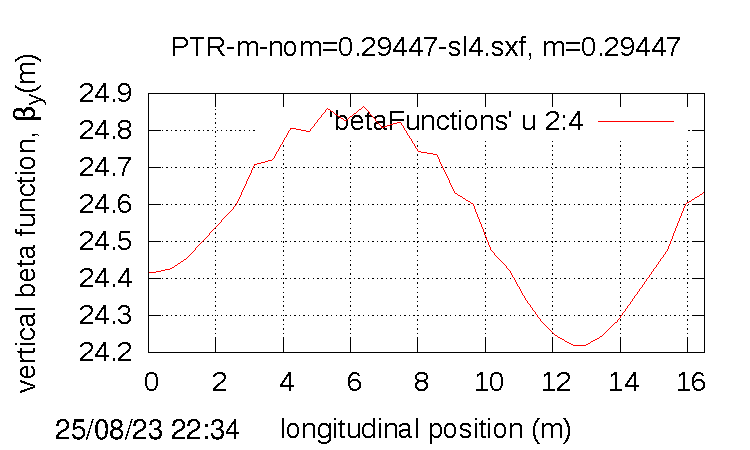
\includegraphics[scale=0.5]{pdf/Fig_II-3.pdf}
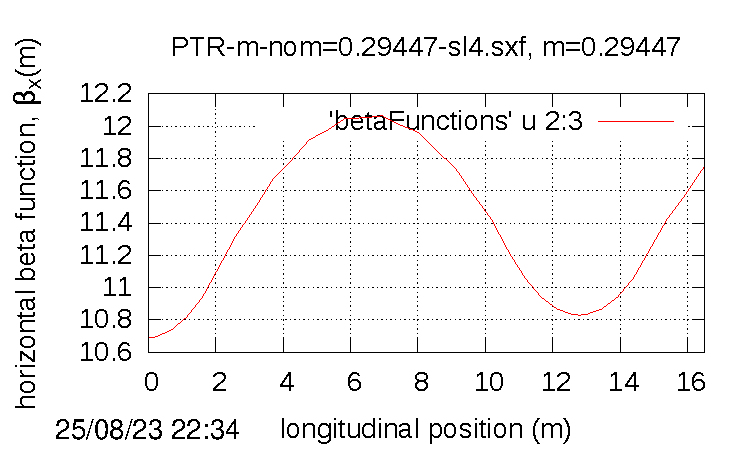
\includegraphics[scale=0.5]{pdf/Fig_II-1.pdf}
\caption{UAL:ETEAPOT results\hfill}
\label{fig:UAL-PTR-m=0.29447}
\end{minipage}
\begin{minipage}[b]{0.49\linewidth}
\centering
\includegraphics[scale=0.5]{/home/talman/Downloads/m-tuning-pdfs/0p29447-quads-off-slightly-over-focused.pdf}
\caption{MAPLE results.\hfill}
\label{fig:MAPLE-PTR-m=0.29447}
\end{minipage}
\end{figure}
%
%
\begin{figure}[htbp]
\hspace{-0.6cm}
\begin{minipage}[b]{0.49\linewidth}
\centering
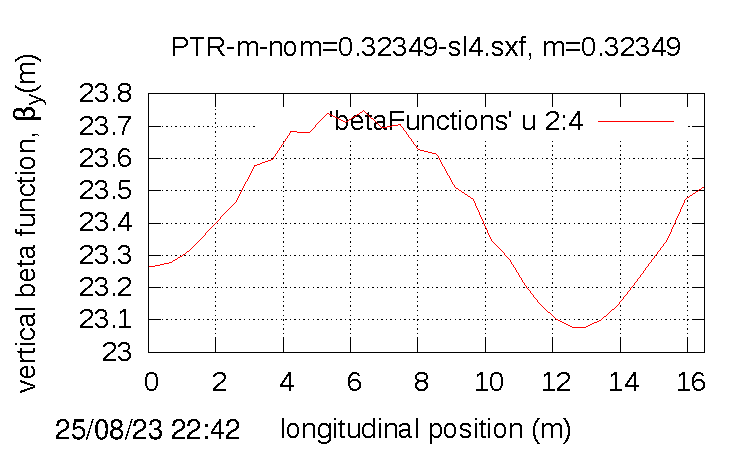
\includegraphics[scale=0.5]{pdf/Fig_II-7.pdf}
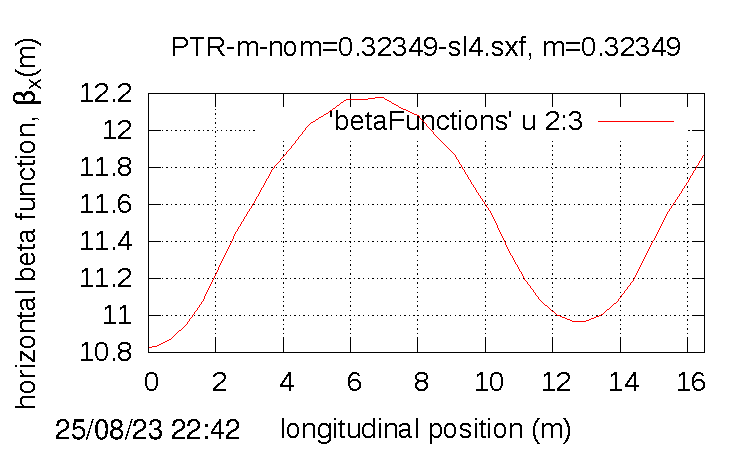
\includegraphics[scale=0.5]{pdf/Fig_II-5.pdf}
\caption{UAL:ETEAPOT results\hfill}
\label{fig:UAL-PTR-m=0.29447}
\end{minipage}
\begin{minipage}[b]{0.49\linewidth}
\centering
\includegraphics[scale=0.5]{/home/talman/Downloads/m-tuning-pdfs/0p32349-quads-off-m-tuned.pdf}
\caption{MAPLE results.\hfill}
\label{fig:MAPLE-PTR-m=0.32349}
\end{minipage}
\end{figure}
%
%
\begin{figure}[htbp]
\hspace{-0.6cm}
\begin{minipage}[b]{0.49\linewidth}
\centering
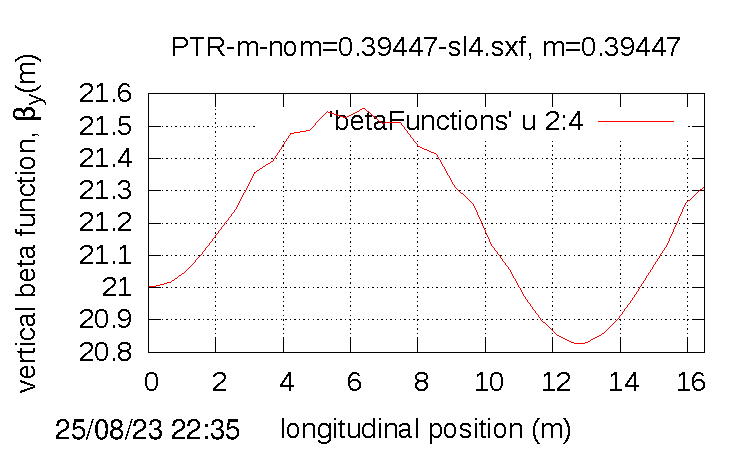
\includegraphics[scale=0.5]{pdf/Fig_II-11.pdf}
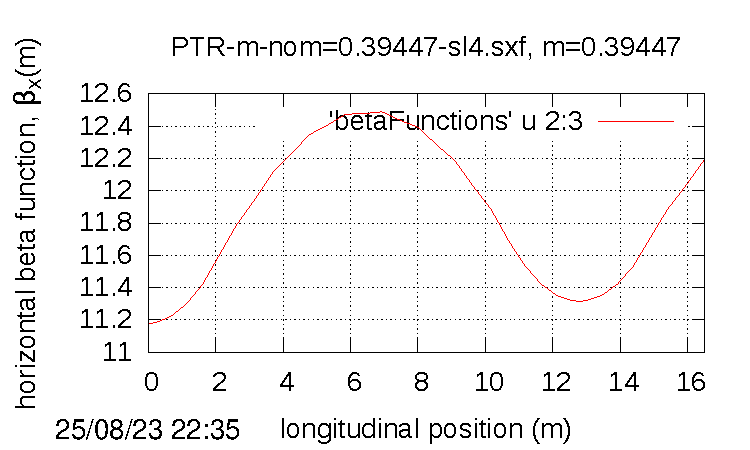
\includegraphics[scale=0.5]{pdf/Fig_II-9.pdf}
\caption{UAL:ETEAPOT results\hfill}
\label{fig:UAL-PTR-m=0.29447}
\end{minipage}
\begin{minipage}[b]{0.49\linewidth}
\centering
\includegraphics[scale=0.5]{/home/talman/Downloads/m-tuning-pdfs/0p39447-quads-off-under-focused.pdf}
\caption{MAPLE results.\hfill}
\label{fig:MAPLE-PTR-m=0.39447}
\end{minipage}
\end{figure}
%

\clearpage

\subsection{Parameters of PTR Benchmark Lattices}  
%
\begin{table}[h]
\centering
\begin{tabular}{|c|c|c|c|c|c|c|c|c|}        \hline
                        & variable name         & unit & {\tt  PTR\_m=0.29447} & {\tt m=0.32349} & {\tt m=0.39447} \\ \hline
cells/arc         & {\tt NCellPerOctant} &        &       1                              &       1                    &        1                   \\
bend radius       &  {\tt r0}                 &  m   &     11.0                           &      11.0                &       11.0               \\
long drift length &  {\tt llsnom}         &  m   &         4.14214                  &     4.14214           &    4.14214            \\
half bend of cell & {\tt lh }                &  r    &         $2\pi$/16                  &      $2\pi$/16        &       $2\pi$/16        \\
half bend length  & {\tt leh}            &  m   &          $2\pi r0$/16             &    $2\pi r0$/16      &       $2\pi r0$/16     \\
circumference     & {\tt circum}      &  m   &         102.252                   &         102.252       &   102.252          \\ \hline
inverse focal length &  {\tt delq}     & 1/m  &     -0.009091                   &       -0.009091       &     -0.009091       \\
field index       &  {\tt m}                 &          &              0.29447             &       0.32349         &      0.39447          \\ \hline
UAL horz beta  & {\tt betax}          &  m    &     $\approx 11.4$           &   $\approx 11.6$  &  $\approx 11.9$    \\
UAL vert beta     & {\tt betay}        &  m    &     $\approx 24.6$           &   $\approx 23.4$  &  $\approx 21.2$    \\ \hline
MAPLE horz beta  & {\tt betax}       &  m    &     $\approx 10$           &   $\approx  10.2$  &  $\approx 10.5$    \\
MAPLE vert beta     & {\tt betay}     &  m    &     $\approx 22$           &   $\approx 21 $  &  $\approx 18.5 $    \\ \hline
horizontal tune  &  {\tt Qx}              &         &                                         &                            &                              \\
vertical tune     &  {\tt Qy}               &         &                                         &                           &                                  \\ \hline
BM-I, horz. tune  &  {\tt Qx}            &         &                 1.42                  &         1.40              &      1.355                  \\
BM-I, vert. tune    &  {\tt Qy}           &         &                 0.655                &         0.655            &      0.76                    \\ 
\hline
\end{tabular}
\caption{\label{tbl:benchmarkParams.1}Parameters of PTR benchmark lattices, including tunes
determined in PTR-benchmark-I investigation for the same three electrode shape parameters, but slightly 
different (though weak) quadrupole strength values.  The two bottom rows are copied from the PTR-BM-I
report.  The (approximate) beta function values are read from the plots above.  They are recorded as
approximate since the rings are only marginally stable.} 
\end{table}
%



\begin{thebibliography}{99}
\bibitem{BenchmarkI}
J.D. Talman and R.M. Talman, \emph{ UAL/ETEAPOT Results 
(Augmented) for Proton EDM Benchmark Lattices,} BNL internal
report, April 29, 2012

\bibitem{ETEAPOT-expanded}
N. Malitsky, J. Talman, and R. Talman, \emph{Appendix UALcode: Development of the
UAL/ETEAPOT Code for the Proton EDM Experiment,} UAL/ETEAPOT documentation
(frequently revised), August, 2012

\bibitem{pEDM}
Storage Ring EDM Collaboration, \emph{A Proposal to Measure the
Proton Electric Dipole Moment with $10^{-29}\,$e-cm Sensitivity,}
especially Appendix 1. October, 2011

\bibitem{Moller}
C. M\o ller, \emph{The Theory of Relativity,} Clarendon Press,
Oxford, 1952, 

\bibitem{Munoz}
G. Mu\~{n}oz and I. Pavic, \emph{A Hamilton-like vector for
the special-relativistic Coulomb problem,} 
Eur. J. Phys. {\bf 27}, 1007-1018, 2006

\bibitem{Talman}
R. Talman, \emph{Geometric Mechanics,} John Wiley and Sons, 2000

\bibitem{Aguirregabiria}
J. Aguirregabiria et al., 
Archiv:physics/0407049v1 [physics.ed-ph] 2004, 

\bibitem{Torkelsson}
U. Torkelsson, Eur. J. Phys., {\bf 19}, 459, 1998, 

\bibitem{Boyer}
T. Boyer, Am. J. Phys. {\bf 72} (8) 992, 2004

\end{thebibliography}
\end{document}




\subsection{Lattice E\_BM\_Z, $m=0$, ``cylindrical'' bending results}
Figures~\ref{fig:UAL_Z_betax} and \ref{fig:RT_Z_betax}
compare $\beta_x$ evaluations
for the ``benchmark'' lattice {\tt E\_BM\_Z\_sl4.sxf}
which has field index $m=0$.
This is the lattice closest to ``cylindrical'' with
lumped quadrupoles just barely strong enough to move
the lattice away from the boundary between vertical
stability and vertical instability.
The figure on the left is evaluated by ETEAPOT, 
the one on the right by the linearized (Wollnik) 
formulas re-derived in an appendix~\cite{pEDM}.
There is agreement to excellent accuracy on local 
beta function dependence $\beta_x(s)$. Similarly good
agreement for vertical beta function $\beta_y(s)$ is exhibited 
in Figures~\ref{fig:UAL_Z_betay} and \ref{fig:RT_Z_betay};
%
\begin{figure}[htbp]
\hspace{-0.6cm}
%
\begin{minipage}[b]{0.5\linewidth}
\centering
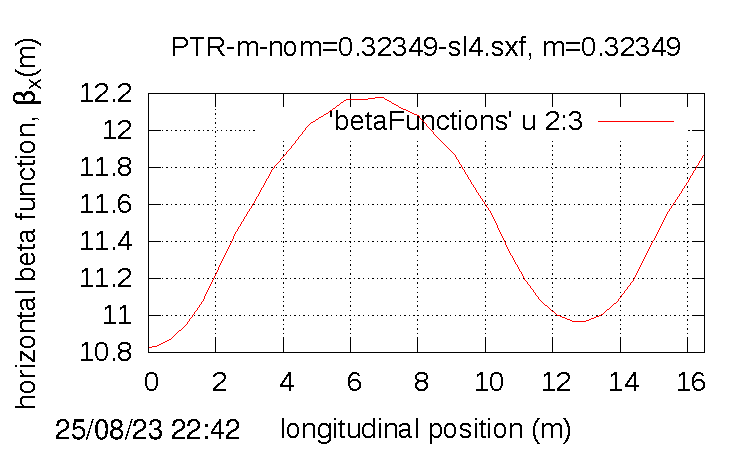
\includegraphics[scale=0.6]{pdf/Fig_II-5.pdf}
\caption{$\beta_x(s)$ calculated by ETEAPOT 
for lattice ``E\_BM\_Z\_sl4''.}
\label{fig:UAL_Z_betax}
\end{minipage}
%
%
\begin{minipage}[b]{0.49\linewidth}
\centering
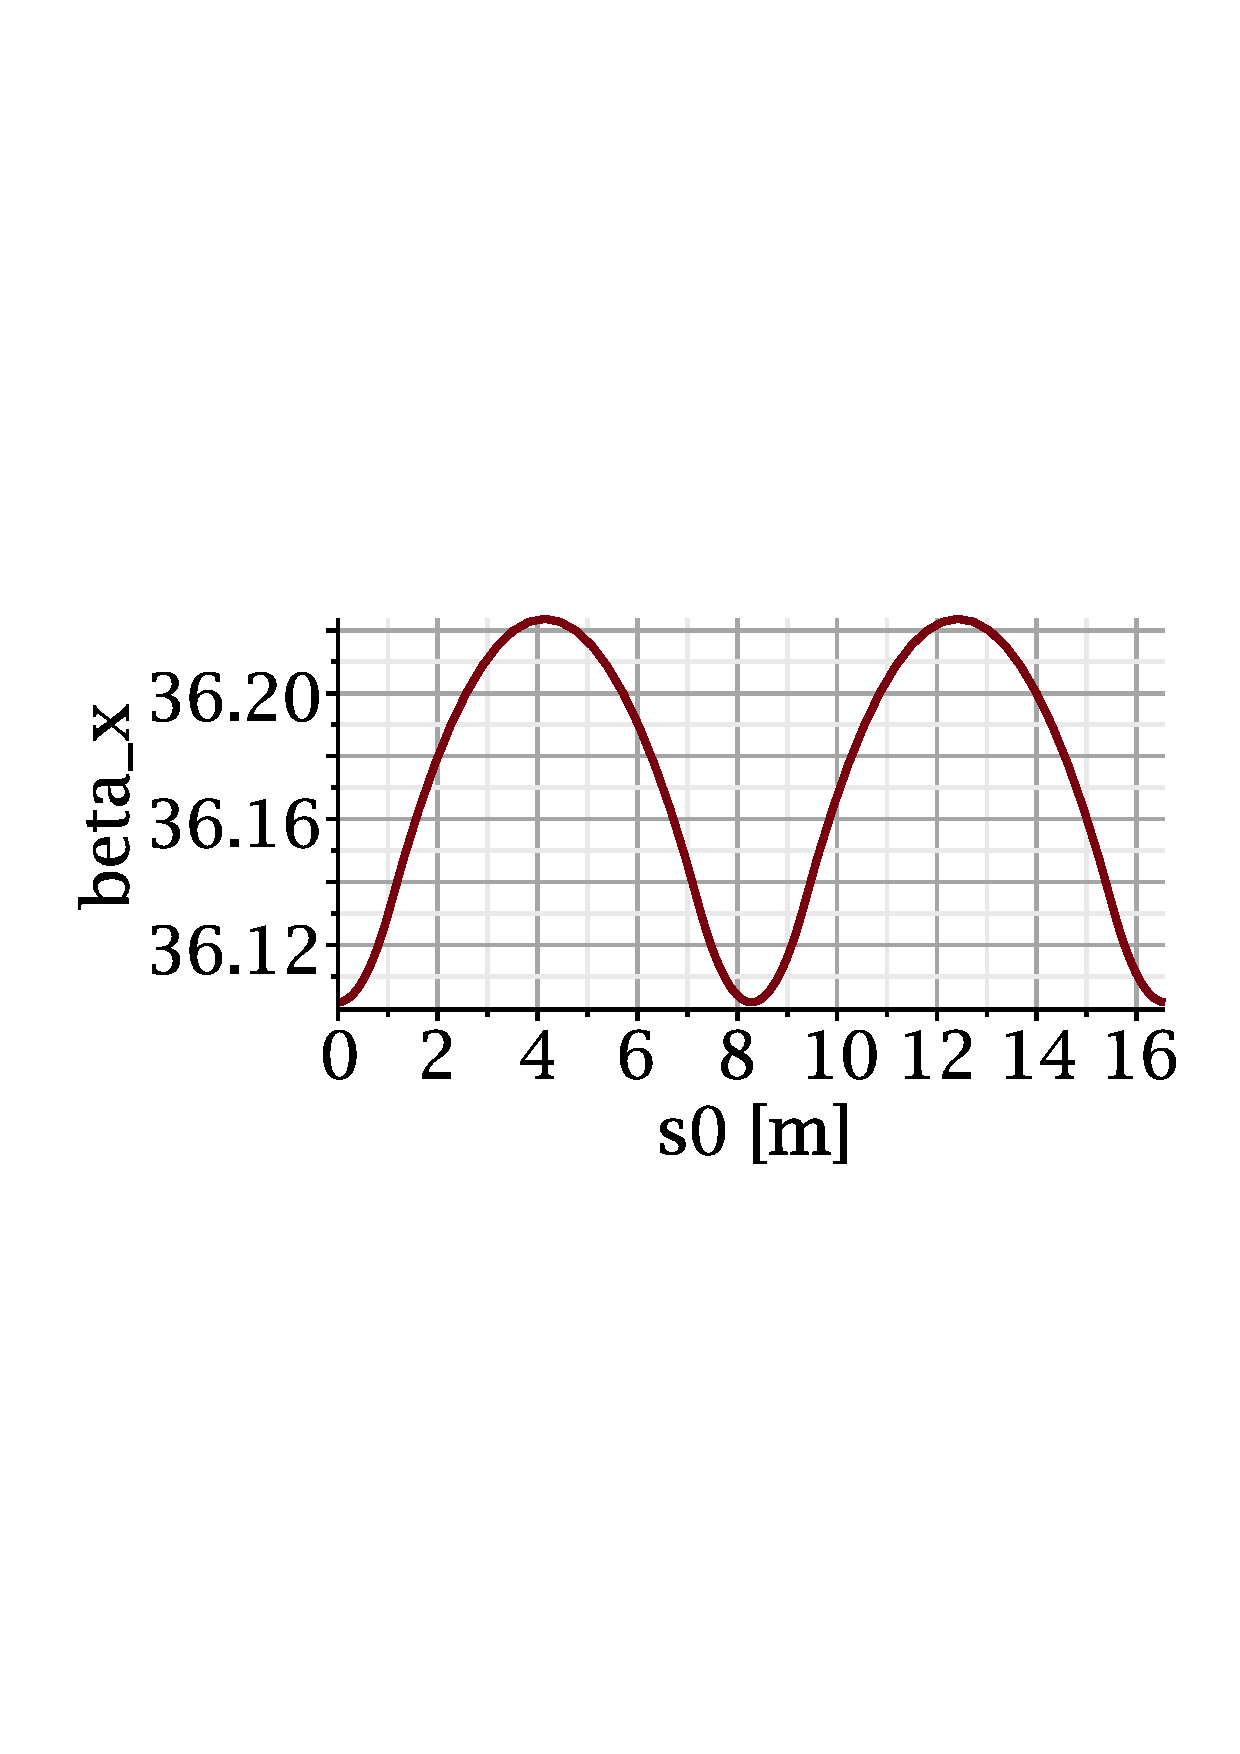
\includegraphics[scale=0.45]{pdf/E_BM_Z_2-betax.pdf}
\caption{$\beta_x(s)$ calculated by MAPLE linearized 
theory for lattice ``E\_BM\_Z\_sl4''.}
\label{fig:RT_Z_betax}
\end{minipage}
%
\end{figure}
%
%
\begin{figure}[htbp]
\hspace{-0.6cm}
\begin{minipage}[b]{0.5\linewidth}
\centering
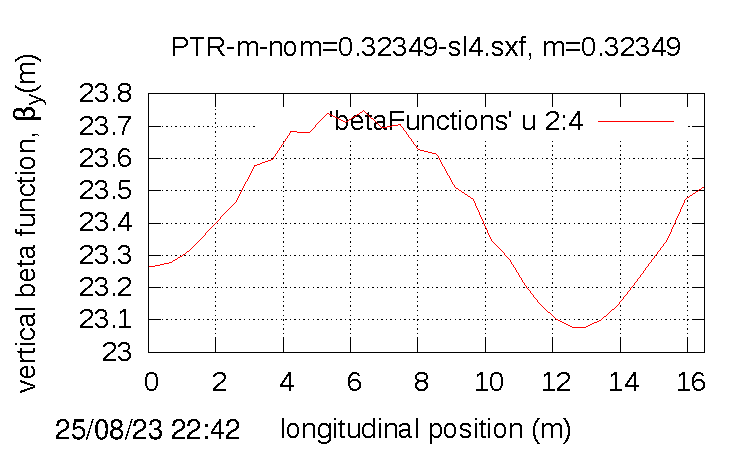
\includegraphics[scale=0.6]{pdf/Fig_II-7.pdf}
\caption{$\beta_y(s)$ calculated by ETEAPOT 
for lattice ``E\_BM\_Z\_sl4''.}
\label{fig:UAL_Z_betay}
\end{minipage}
%
%
\begin{minipage}[b]{0.49\linewidth}
\centering
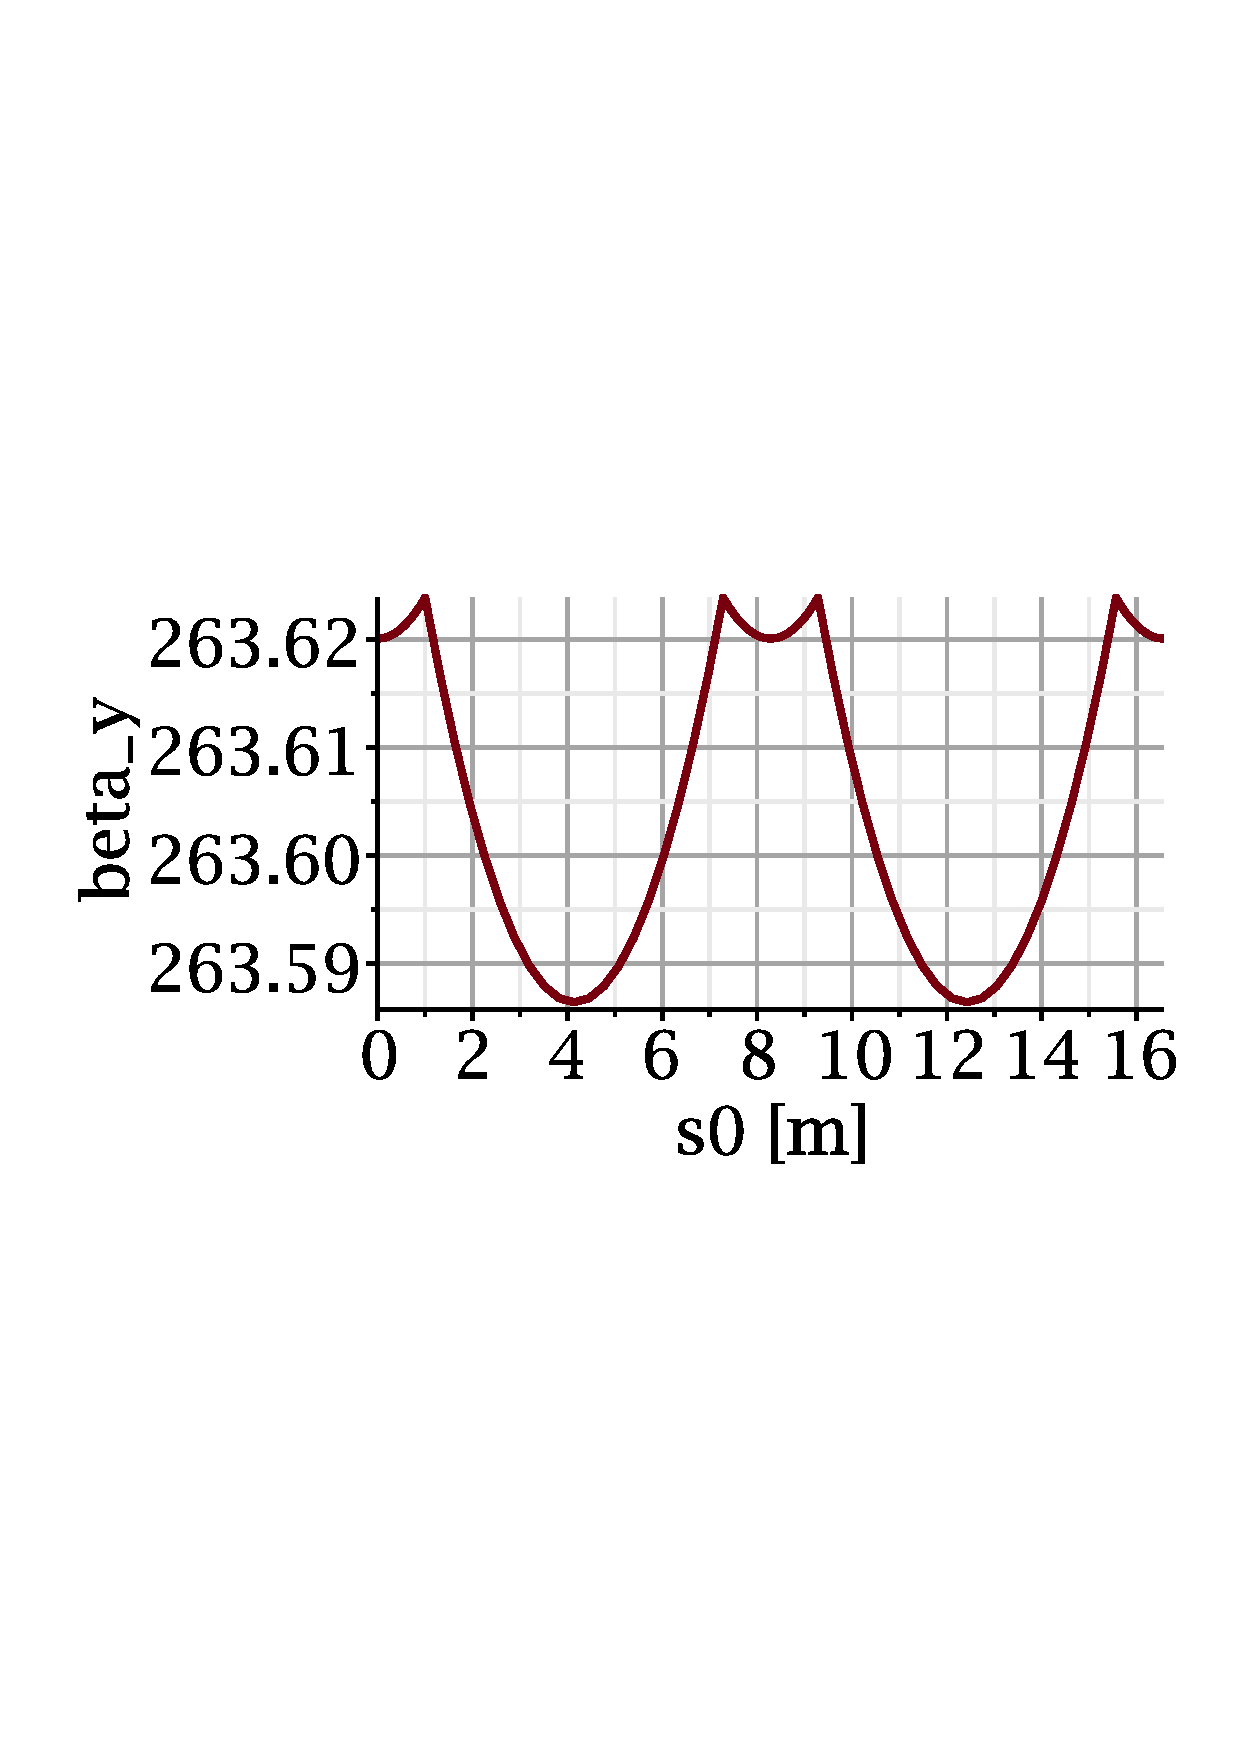
\includegraphics[scale=0.45]{pdf/E_BM_Z_2-betay.pdf}
\caption{$\beta_y(s)$ calculated by MAPLE linearized 
theory for lattice ``E\_BM\_Z\_sl4''.}
\label{fig:RT_Z_betay}
\end{minipage}
\end{figure}
%

\subsection{Lattice E\_BM\_M1.0, $m=-1$, bending results}
Figures~\ref{fig:UAL_M1.0_betax} through \ref{fig:RT_M1.0_betay}
contain evaluations
for the ``benchmark'' lattice {\tt E\_BM\_M1.0\_sl4.sxf}. 
which has field index $m=-1$; in this case the radial electric
field $E_r$ is independent of radial displacement $x\approx r-r_0$.
Agreement is again excellent.
%
\begin{figure}[htbp]
\hspace{-0.6cm}
\begin{minipage}[b]{0.49\linewidth}
\centering
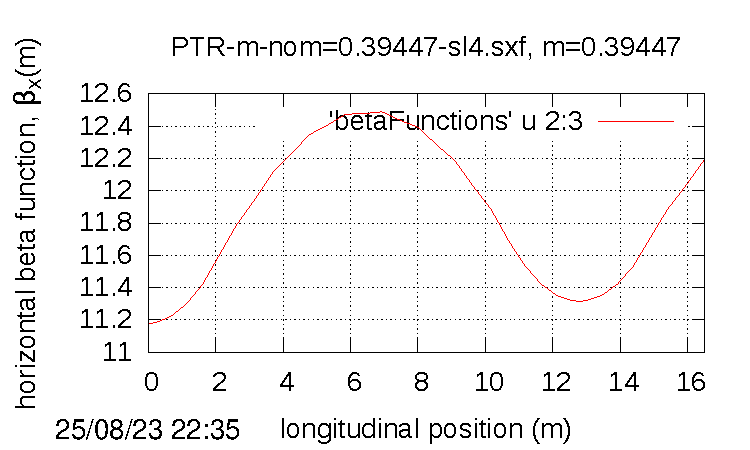
\includegraphics[scale=0.6]{pdf/Fig_II-9.pdf}
\caption{$\beta_x$ calculated by ETEAPOT 
for lattice ``E\_BM\_M1.0\_sl4''.}
\label{fig:UAL_M1.0_betax}
\end{minipage}
%
%
\begin{minipage}[b]{0.49\linewidth}
\centering
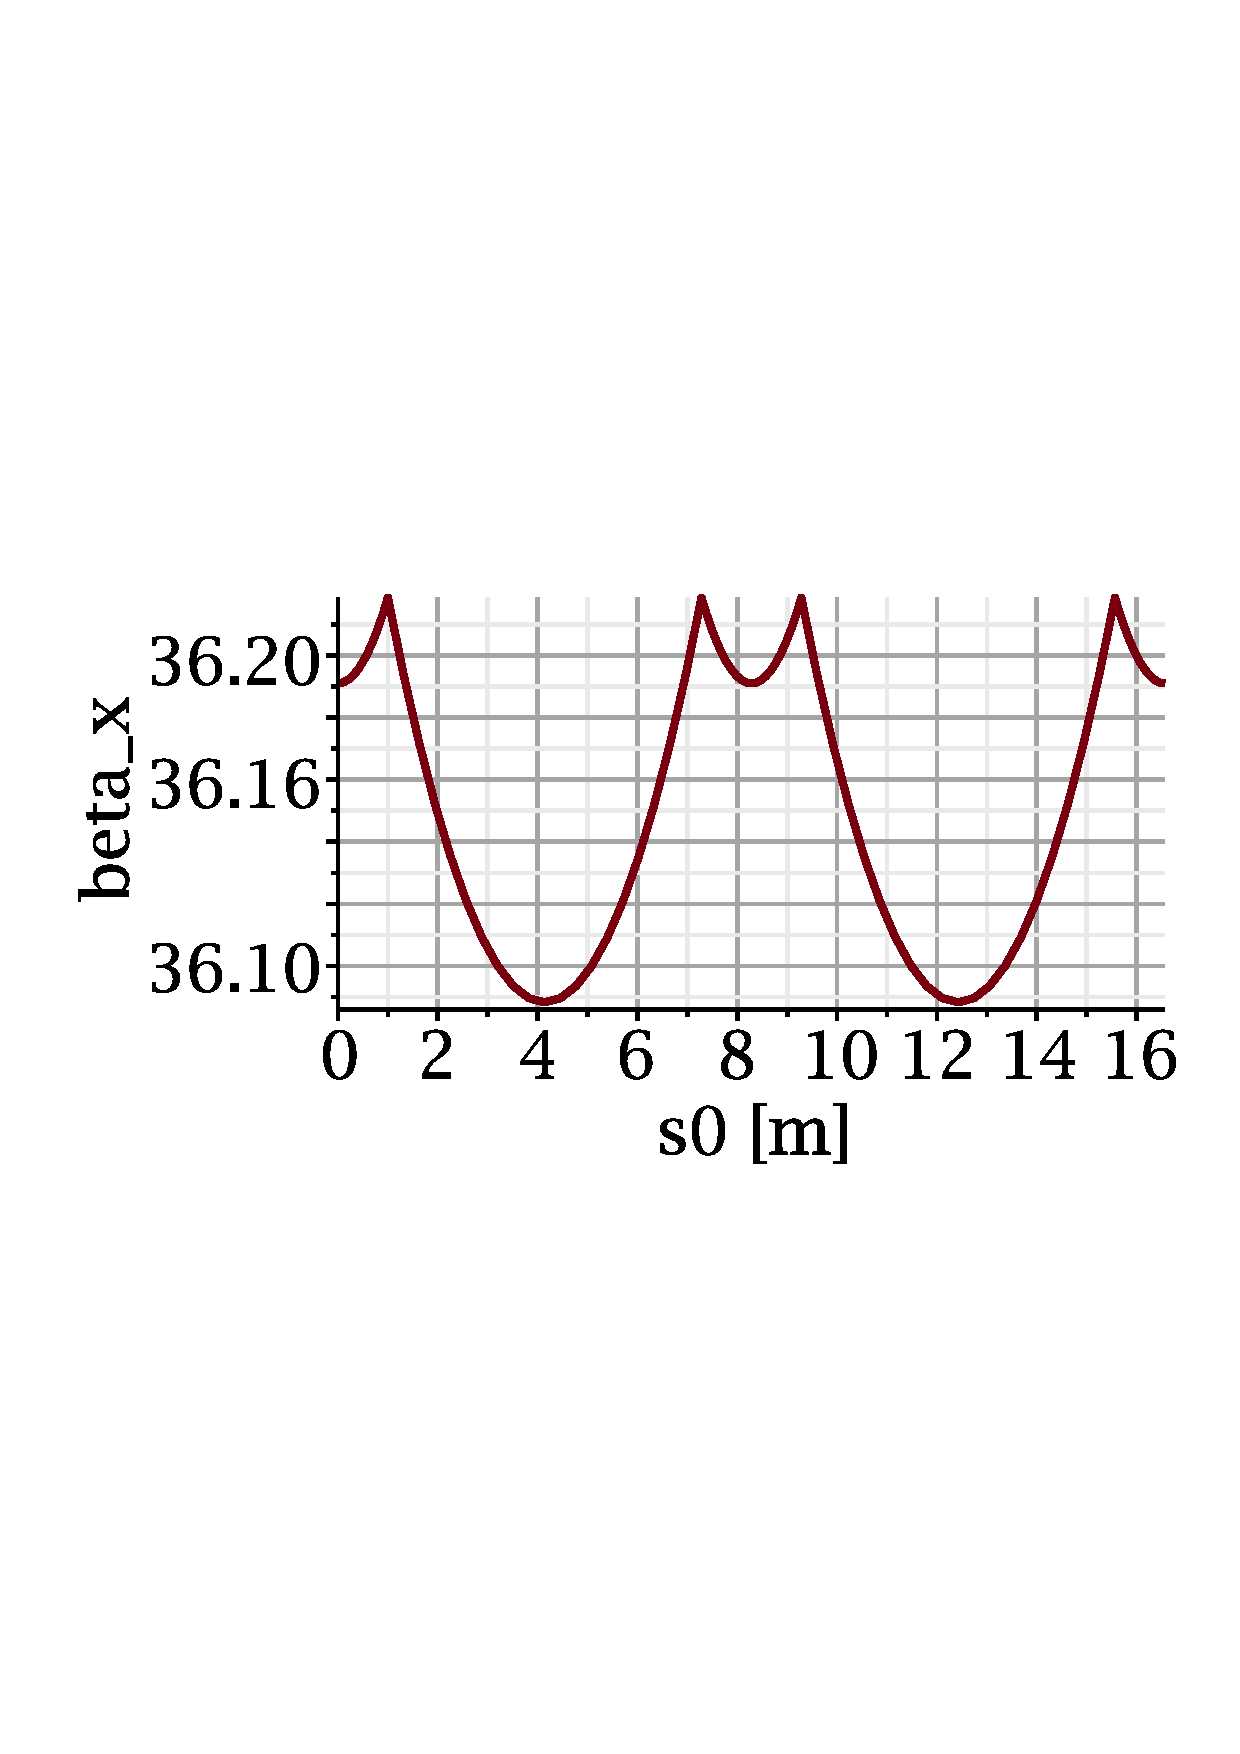
\includegraphics[scale=0.45]{pdf/E_BM_P1p0_2-betax.pdf}
\caption{$\beta_x$ calculated by MAPLE linearized 
theory for lattice ``E\_BM\_M1.0\_sl4''.}
\label{fig:RT_M1.0_betax}
\end{minipage}
\end{figure}
%
%
\begin{figure}[htbp]
\hspace{-0.6cm}
\begin{minipage}[b]{0.49\linewidth}
\centering
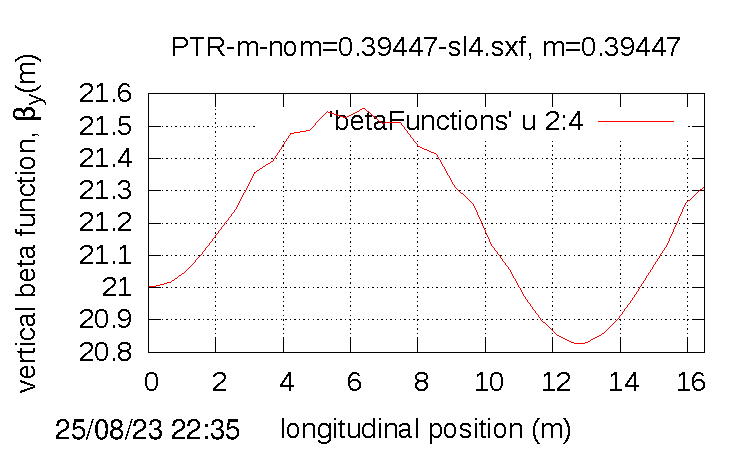
\includegraphics[scale=0.6]{pdf/Fig_II-11.pdf}
\caption{$\beta_y$ calculated by ETEAPOT 
for lattice ``E\_BM\_M1.0\_sl4''.}
\label{fig:UAL_M1.0_betay}
\end{minipage}
%
%
\begin{minipage}[b]{0.49\linewidth}
\centering
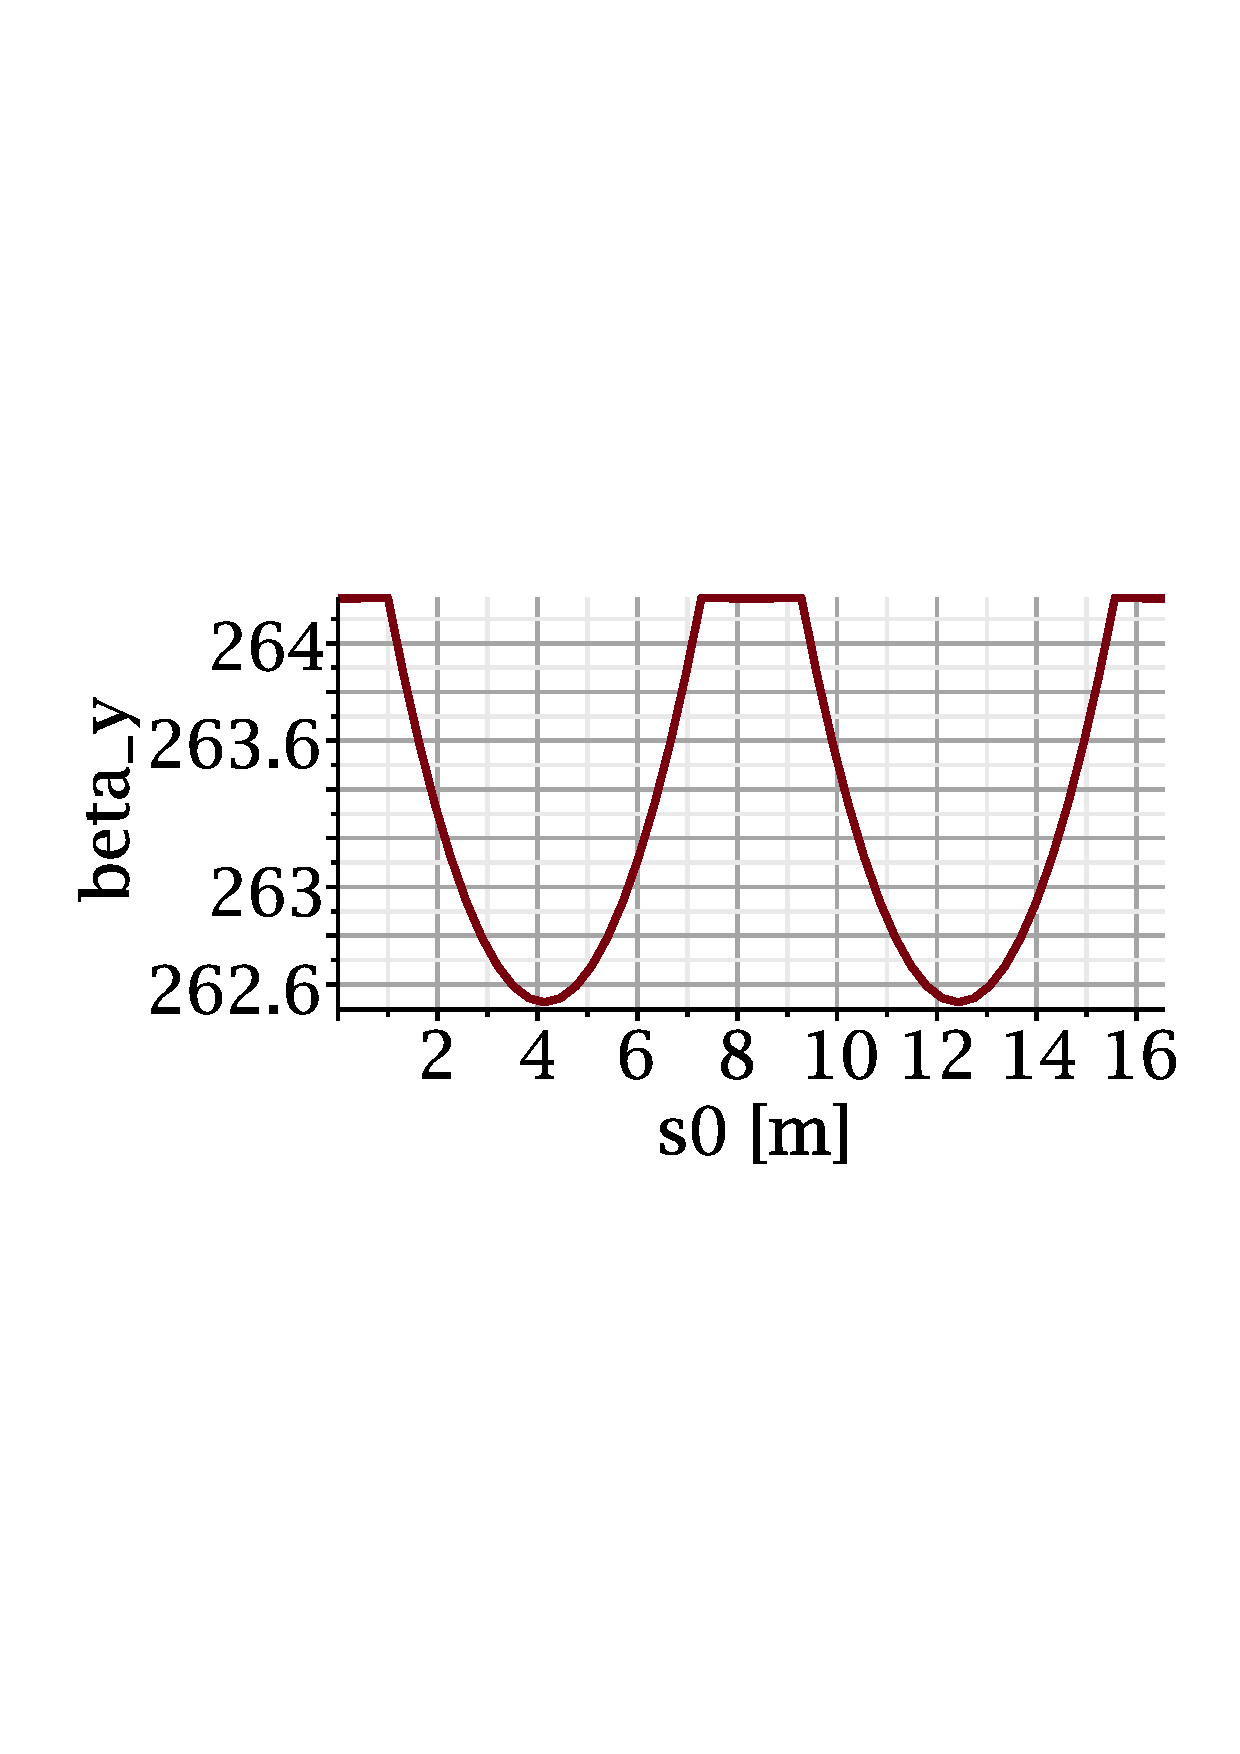
\includegraphics[scale=0.45]{pdf/E_BM_M1p0_2-betay.pdf}
\caption{$\beta_y$ calculated by linearized 
theory for lattice ``E\_BM\_M1.0\_sl4''.}
\label{fig:RT_M1.0_betay}
\end{minipage}
\end{figure}
%

Figure~\ref{fig:SliceCompare} compares different
ETEAPOT results for lattices {\tt E\_BM\_Z\_sl4.sxf}
and {\tt E\_BM\_Z.sxf}. These are actually the identical
lattice treated two different ways. The ``\_sl4''
suffix in the first file name indicates that the
bend elements have been split into four slices in
the (external) {\tt sxf} file. In the other case the
bends split into the same four slices, but 
ETEAPOT performs the slicing (internally) called for
by the {\tt splitForBends=2} parameter. The apparent
disagreement is caused by a bug in the plotting procedure
which joins points by straight lines. NOTE to JDT: 
either we fix the bug or suppress the plot? The actual
beta function evaluations agree perfectly, at least to
the accuracy of the plot.
%
\begin{figure}[h]
\centering
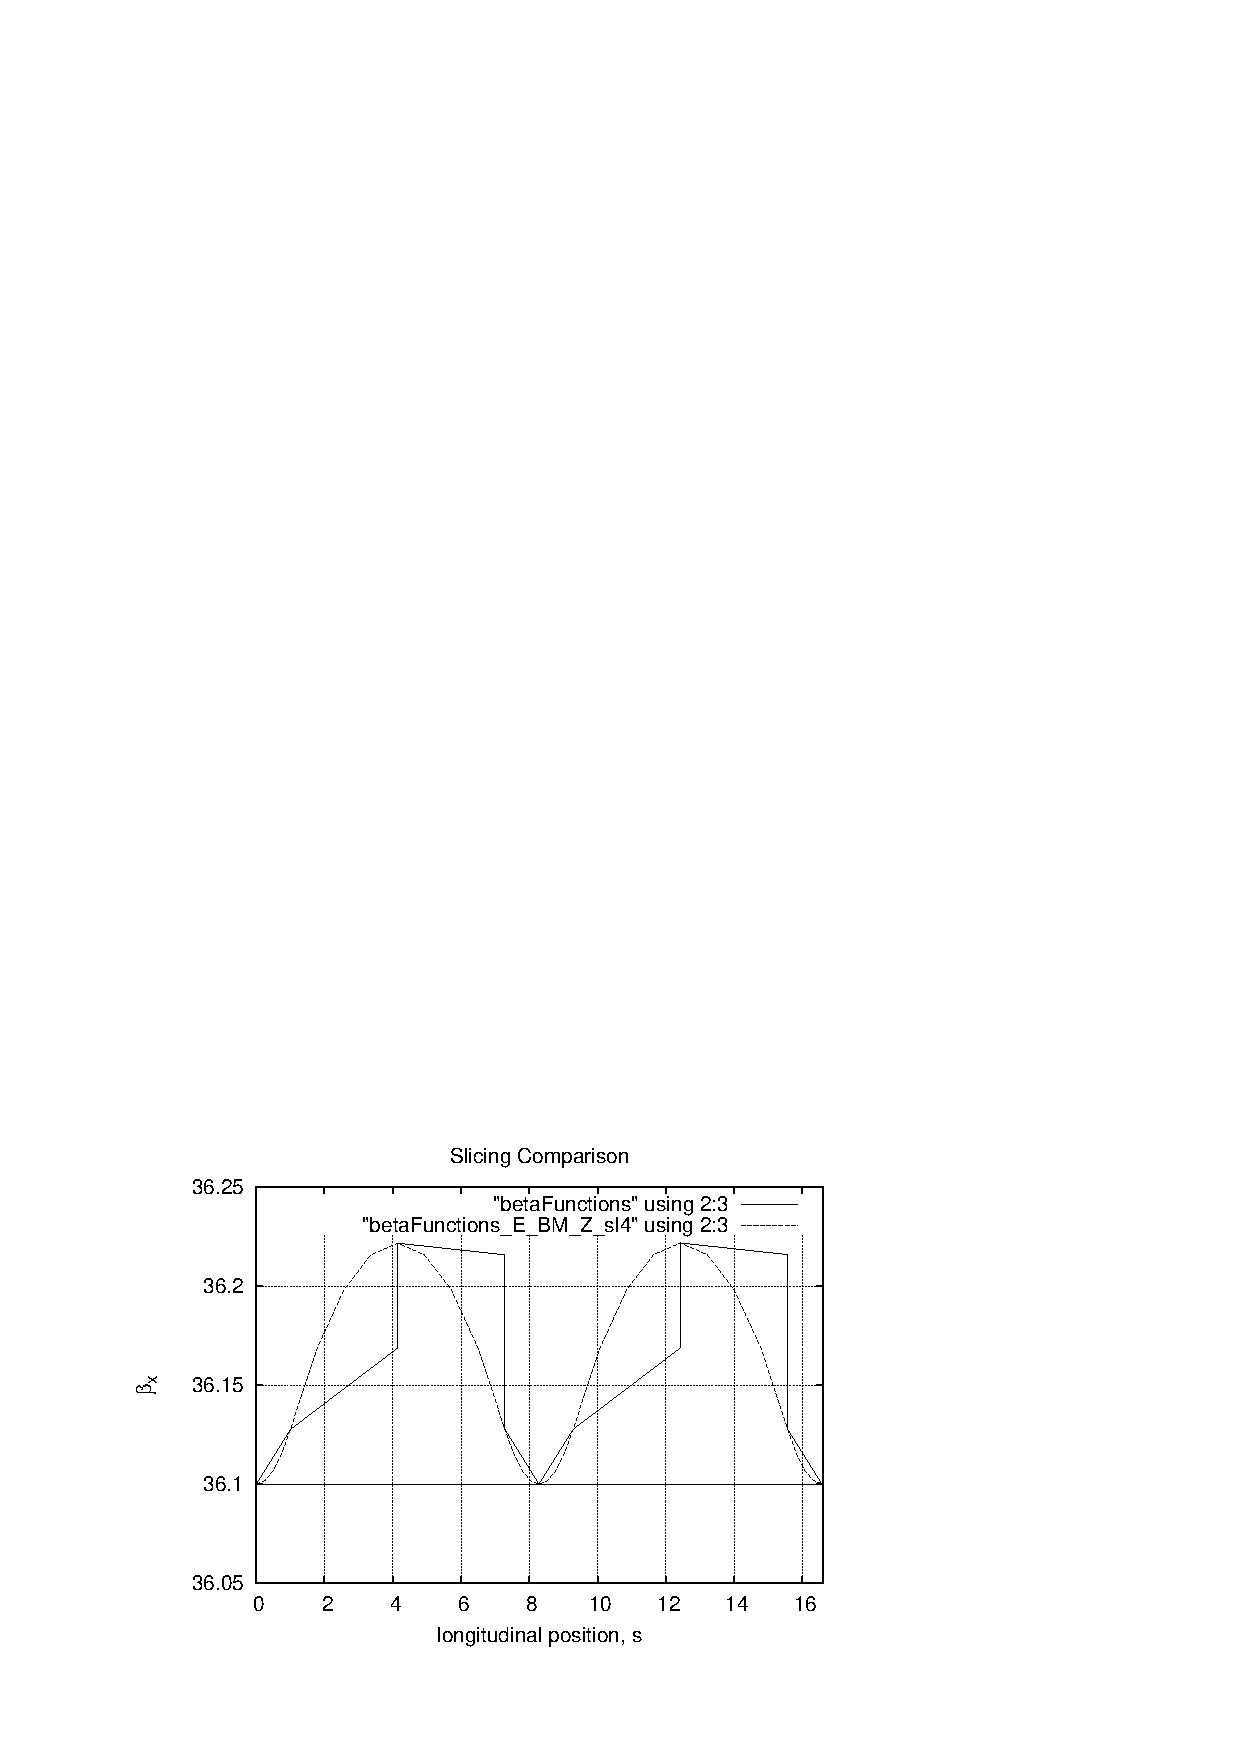
\includegraphics[scale=0.6]{pdf/SliceCompare.pdf}
\caption{\label{fig:SliceCompare}Comparison of external slicing
(via the {\tt sxf} file) and UAL-internal slicing, via the 
{\tt splitForBends=2} parameter. Only selected points (connected 
by straight lines) are plotted in the internal slicing case. 
This accounts for the different local appearance of the plots.}
\end{figure}
%
Table~\ref{tbl:PTR-benchmarkParams.1} contains PTR  parameters, for the three PTR benchmark lattices.
including tune values determined in PTR Benchmark-I report.


%
\begin{table}[h]
\centering
\begin{tabular}{|c|c|c|c|c|c|c|c|c|}           \hline
file name         & variable name     & unit  &   linearized  & 2 slices/bend &       \\ \hline
cells/arc         & {\tt NCellPerArc} &       &        20     &  &        \\
bend radius       &  {\tt r0}         &  m    &       40.0    &  &        \\
half drift length &  {\tt Ldh}        &  m    &        1.0    &  &        \\
half bend per cell & {\tt Thetah}     &  r    &  0.078539816  &  &        \\
half bend length  & {\tt Leh}         &  m    &   3.141592    &  &        \\
circumference     & {\tt circum}      &  m    &    331.327    &  &        \\ 
inverse focal length &  {\tt q}       & 1/m   &     0.0019075 &  &        \\
field index       &  {\tt m}          &       &         1.0   &  &         \\ \hline
horizontal beta  & {\tt betax}       &  m    &     36.1910   &  36.1910 &         \\ \hline
vertical beta     & {\tt betay}       &  m    &     262.237   &  262.2370 &         \\ \hline
horizontal tune  &  {\tt Qx}         &       &      1.4588   &  1.4588 &         \\   \hline
vertical tune     &  {\tt Qy}         &       &     0.20047   &  0.2005 &         \\  \hline
\end{tabular}
\caption{\label{tbl:PTR-benchmarkParams.1}E\_TEAPOT oarameters for PTR.}
\end{table}
%
%
\begin{table}[h]
\caption{\label{tbl:benchmarkParams.Z}E\_TEAPOTComparisons for {\tt E\_BM\_Z.sxf}.
} 
\medskip
\centering
\begin{tabular}{|c|c|c|c|c|c|c|c|c|}           \hline
file name         & variable name     & unit  &  linearized  & 2 slices/bend  &     \\ \hline
cells/arc         & {\tt NCellPerArc} &       &       20     &   &     \\
bend radius       &  {\tt r0}         &  m    &      40.0    &   &     \\
half drift length &  {\tt Ldh}        &  m    &     1.0      &   &     \\
half bend per cell & {\tt Thetah}     &  r    &  0.078539816 &   &     \\
half bend length  & {\tt Leh}         &  m    &  3.141592    &   &     \\
circumference     & {\tt circum}      &  m    &   331.327    &   &     \\ 
inverse focal length &  {\tt q}       & 1/m   & -0.00005960  &   &     \\
field index       &  {\tt m}          &       &  1.0e-10     &   &     \\ \hline
horizontal beta  & {\tt betax}       &  m    &  36.1018     &   36.0795 &     \\ \hline
vertical beta     & {\tt betay}       &  m    &  263.620     &   261.4688 &     \\ \hline
horizontal tune  &  {\tt Qx}         &       &   1.4578     &   1.4581 &     \\ \hline
vertical tune     &  {\tt Qy}         &       &   0.20004    &   0.2018 &     \\
\hline
\end{tabular}
\end{table}
%

%
\begin{table}[h]
\caption{\label{tbl:benchmarkParams.M1.0}E\_TEAPOT comparisons for {\tt E\_BM\_M1.0.sxf}
} 
\medskip
\centering
\begin{tabular}{|c|c|c|c|c|c|c|c|c|}           \hline
file name         & variable name     & unit & linearized    & 2 slices/bend &    \\ \hline
cells/arc         & {\tt NCellPerArc} &      &      20       &  &    \\
bend radius       &  {\tt r0}         &  m   &     40.0      &  &    \\
half drift length &  {\tt Ldh}        &  m   &      1.0      &  &    \\
half bend per cell & {\tt Thetah}     &  r   &   0.078539816 &  &    \\
half bend length  & {\tt Leh}         &  m   &    3.141592   &  &    \\
circumference     & {\tt circum}      &  m   &   331.327     &  &    \\
inverse focal length &  {\tt q}       & 1/m  &    -0.002019  &  &    \\ 
field index       &  {\tt m}          &      &     -1.0      &  &    \\ \hline
horizontal beta  & {\tt betax}       &  m   &    35.9237    &  35.8566 &    \\ \hline
vertical beta     & {\tt betay}       &  m   &   264.182     &  251.8522 &    \\ \hline
horizontal tune  &  {\tt Qx}         &      &     1.4605    &  1.4620 &    \\ \hline
vertical tune     &  {\tt Qy}         &      &     0.20024   &  0.2102 &    \\
\hline
\end{tabular}
\end{table}
%

